\documentclass[9pt,a4paper]{extarticle}
\usepackage[utf8]{inputenc}
\usepackage[spanish]{babel}
\usepackage[top=0.4in, bottom=0.4in, left=0.5in, right=0.75in]{geometry}
\usepackage{amsmath, amssymb, amsfonts}
\usepackage{graphicx}

%letra en arial
%\usepackage{helvet}
%\renewcommand{\familydefault}{\sfdefault}

\usepackage{enumerate}% http://ctan.org/pkg/enumerate
\newcommand{\plus}{\scalebox{0.6}{$+$}}

\begin{document}

\begin{enumerate}
    \item Calcular el potencial eléctrico y el vector campo eléctrico en el punto P con los siguientes datos: \\[0.6cm]
    \begin{minipage}{0.4\textwidth}
\begin{flushright} 
$$q_1=2\mu C$$
$$q_2=-4\mu C$$
$$q_3=2 \mu C$$
\end{flushright}
\end{minipage}
~
\begin{minipage}{0.4\textwidth}
\begin{flushleft} 
    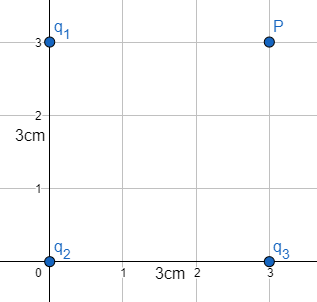
\includegraphics[scale=0.3]{punto1.png}
\end{flushleft}
\end{minipage}

    \item Una esfera de masa $10 g$ y carga de $20\mu C$ se encuentra colgadade un hilo, el cual está adherido a un plano vertical (infinito) cuya densidad superficial de carga es $20\dfrac{nC}{cm^2}$. Se pide calcular el ángulo  que el hilo forma con la vertical y la tensión del hilo.
    \item Un protón es acelerado, a partir del reposo, a través de una diferencia de potencial de $100V$. Si se sabe que su energía cinética es de $50 eV$, que la masa es $1,6725 \times 10^{-27} kg$ y $q=1,6 \times 10^{-19} C$. Se desea saber la velocidad final del protón.
    \item Un protón con una velocidad de $3\times10^5 \dfrac{m}{s}$ en el sentido positivo de las $x$, ingresa a una región del espacio en la que existe un campo magnético $B$ cuyas componentes son $0,3 T$ (eje $x$) y $0,2 T$ (eje $y$). Calcular la fuerza total sobre el protón. ($m = 1,6725 \times 10^{-27}kg$ y $g = 1,6 \times 10^{-19} C$, tomar $g=10\dfrac{m}{s^2}$).
    \item Un conductor recto e indefinido transporta una intensidad de corriente eléctrica de $2A$. Se desea calcular la intensidad del campo magnético $B$, su dirección y sentido, generado en un punto P ubicado a $20 cm$ del conductor.
    
\end{enumerate}


\end{document}